Until very recently, \dis has been the one process mostly determining \pdf{}s
on its own, even though a non-negligible fraction of \acrfull{ftdy} data was
already included in the main fits.
%
With the advent of the \acrfull{lhc}, this started changing, since the
incredible amount of data generated (and those that will be produced in the
future) are compensating the indirectness of the probe.
%
The \nnpdfr{4.0} release shown for the first time how the \lhc data are not
only giving sizeable contribution to the \pdf{}s determination, but also able
to constraint the \pdf{}s shape on their own \cite{Ball:2021leu}, to a
remarkable degree of accuracy.

\begin{figure}
	\centering
	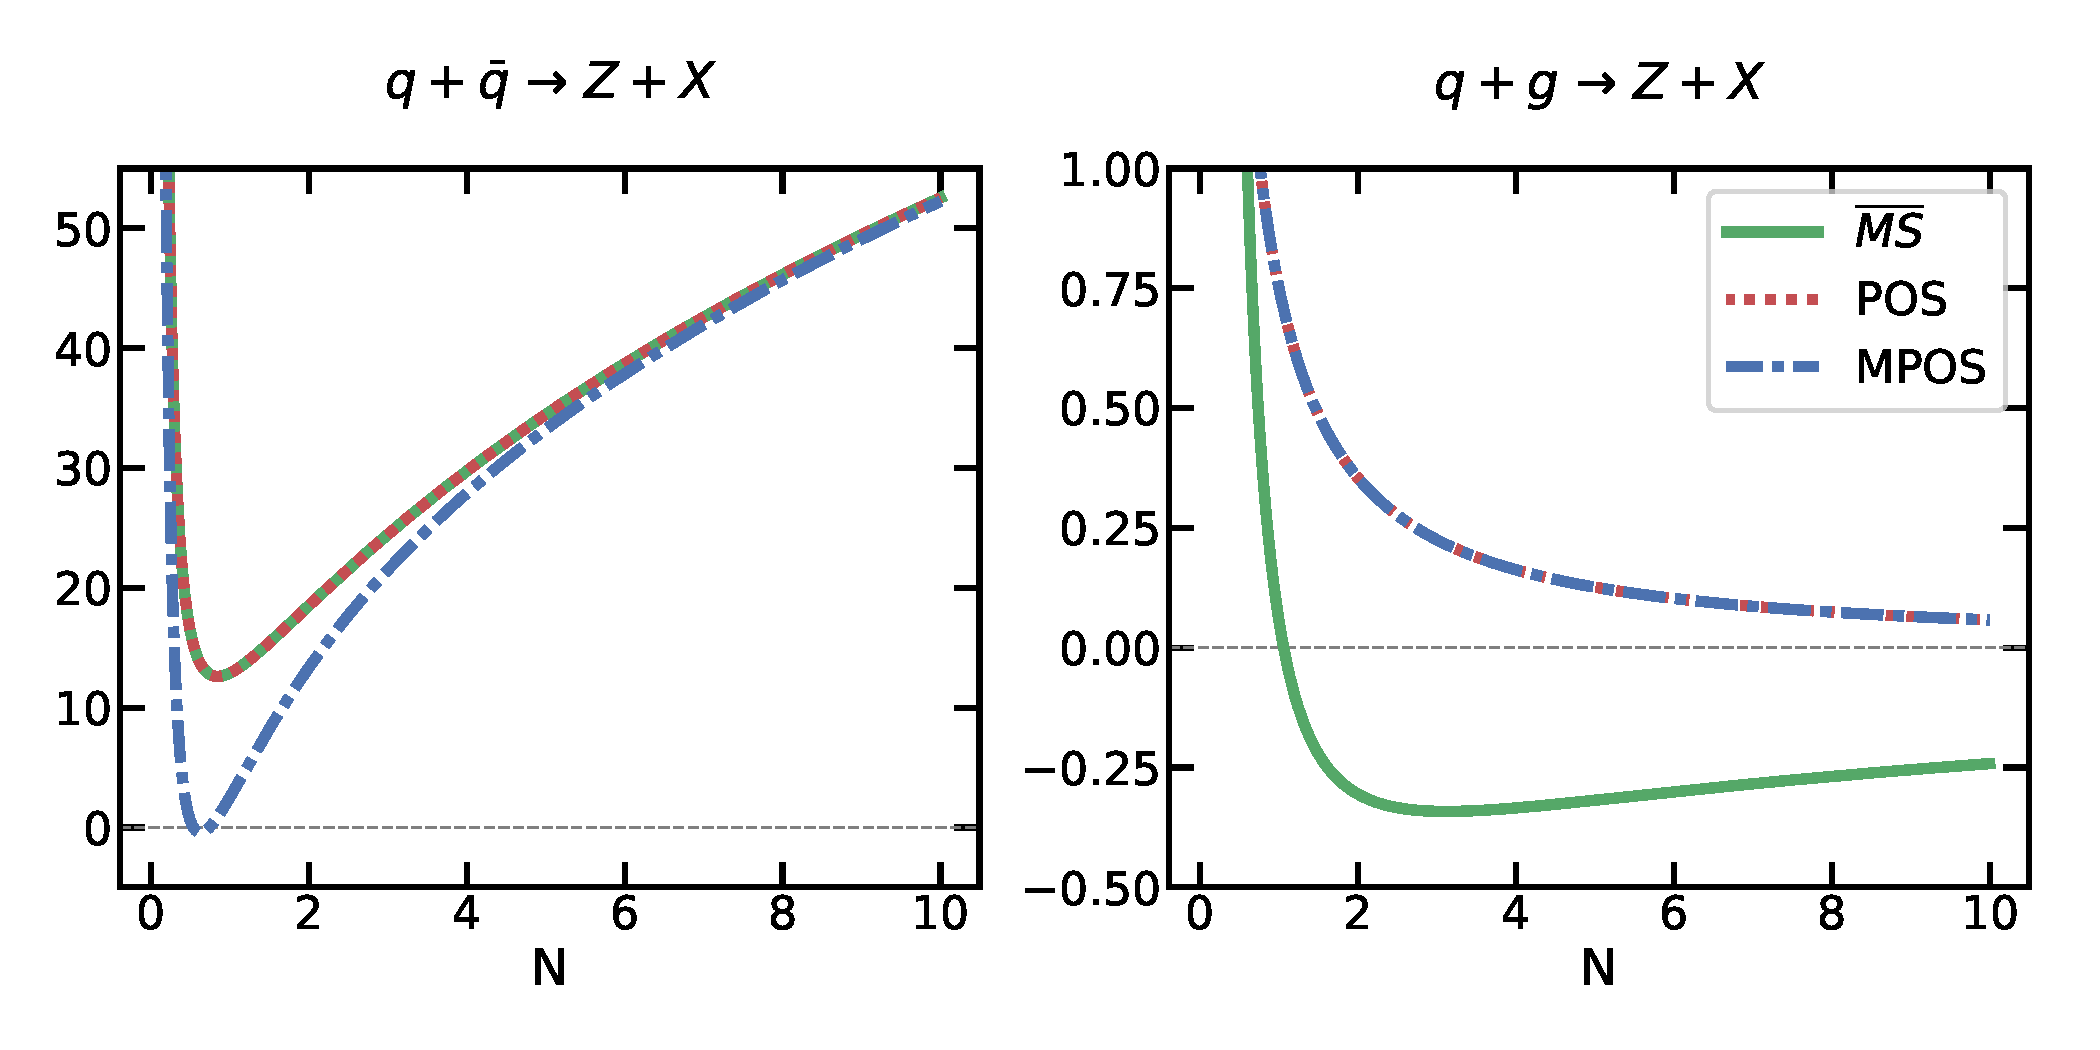
\includegraphics[width=0.6\textwidth]{ch-qcd/dy}
	\caption{
		The \lo Feynman diagram associated to the scattering of two quark
		components of the proton in the $s$-channel, generating a virtual \ew
		boson, eventually decaying leptonically.
	}
	\label{fig:qcd/dy}
\end{figure}

For this reason, double hadronic initiated processes, like $pp$ at \lhc, or
$p\bar{p}$ at \tevatron, are now a relevant part of the global \qcd dataset
used in \pdf{}s extraction.
%
But while for the \dis process analytical calculations are available, most
double hadronic processes require the usage of \acrfull{mc} integrators, since
the resulting integrals are not known analytically, and they quickly extend to
many dimensions.
%
Then, in order to obtain the theory predictions required in \pdf fits, many
different codes are required, since no one implements all possible processes at
the state-of-the-art perturbative order (usually \nnlo by now, but only for
more common processes), and no one is optimal for all of them.

This wide landscape of theoretical predictions, involving increasingly more
demanding software tools, is a challenge for a global \qcd fits, like \pdf
ones, since they will need to interface with a variety of codes constantly
evolving, and find an effective way to decouple the fit itself from the
computational costs involved.
%
This is why interpolation grids have been introduced, to store the results of
\mc computations and offer a unique and fast interface for their consumption.
Grids will be described in more details in \cref{ch:pine}, where a new grid
layout, \pineappl \cite{Carrazza:2020gss}, initially motivated by the extension
of existing formats to allow \ew corrections, has been used to construct a full
pipeline to streamline the process of producing predictions for \pdf and
similar fits.

\begin{figure}
	\centering
	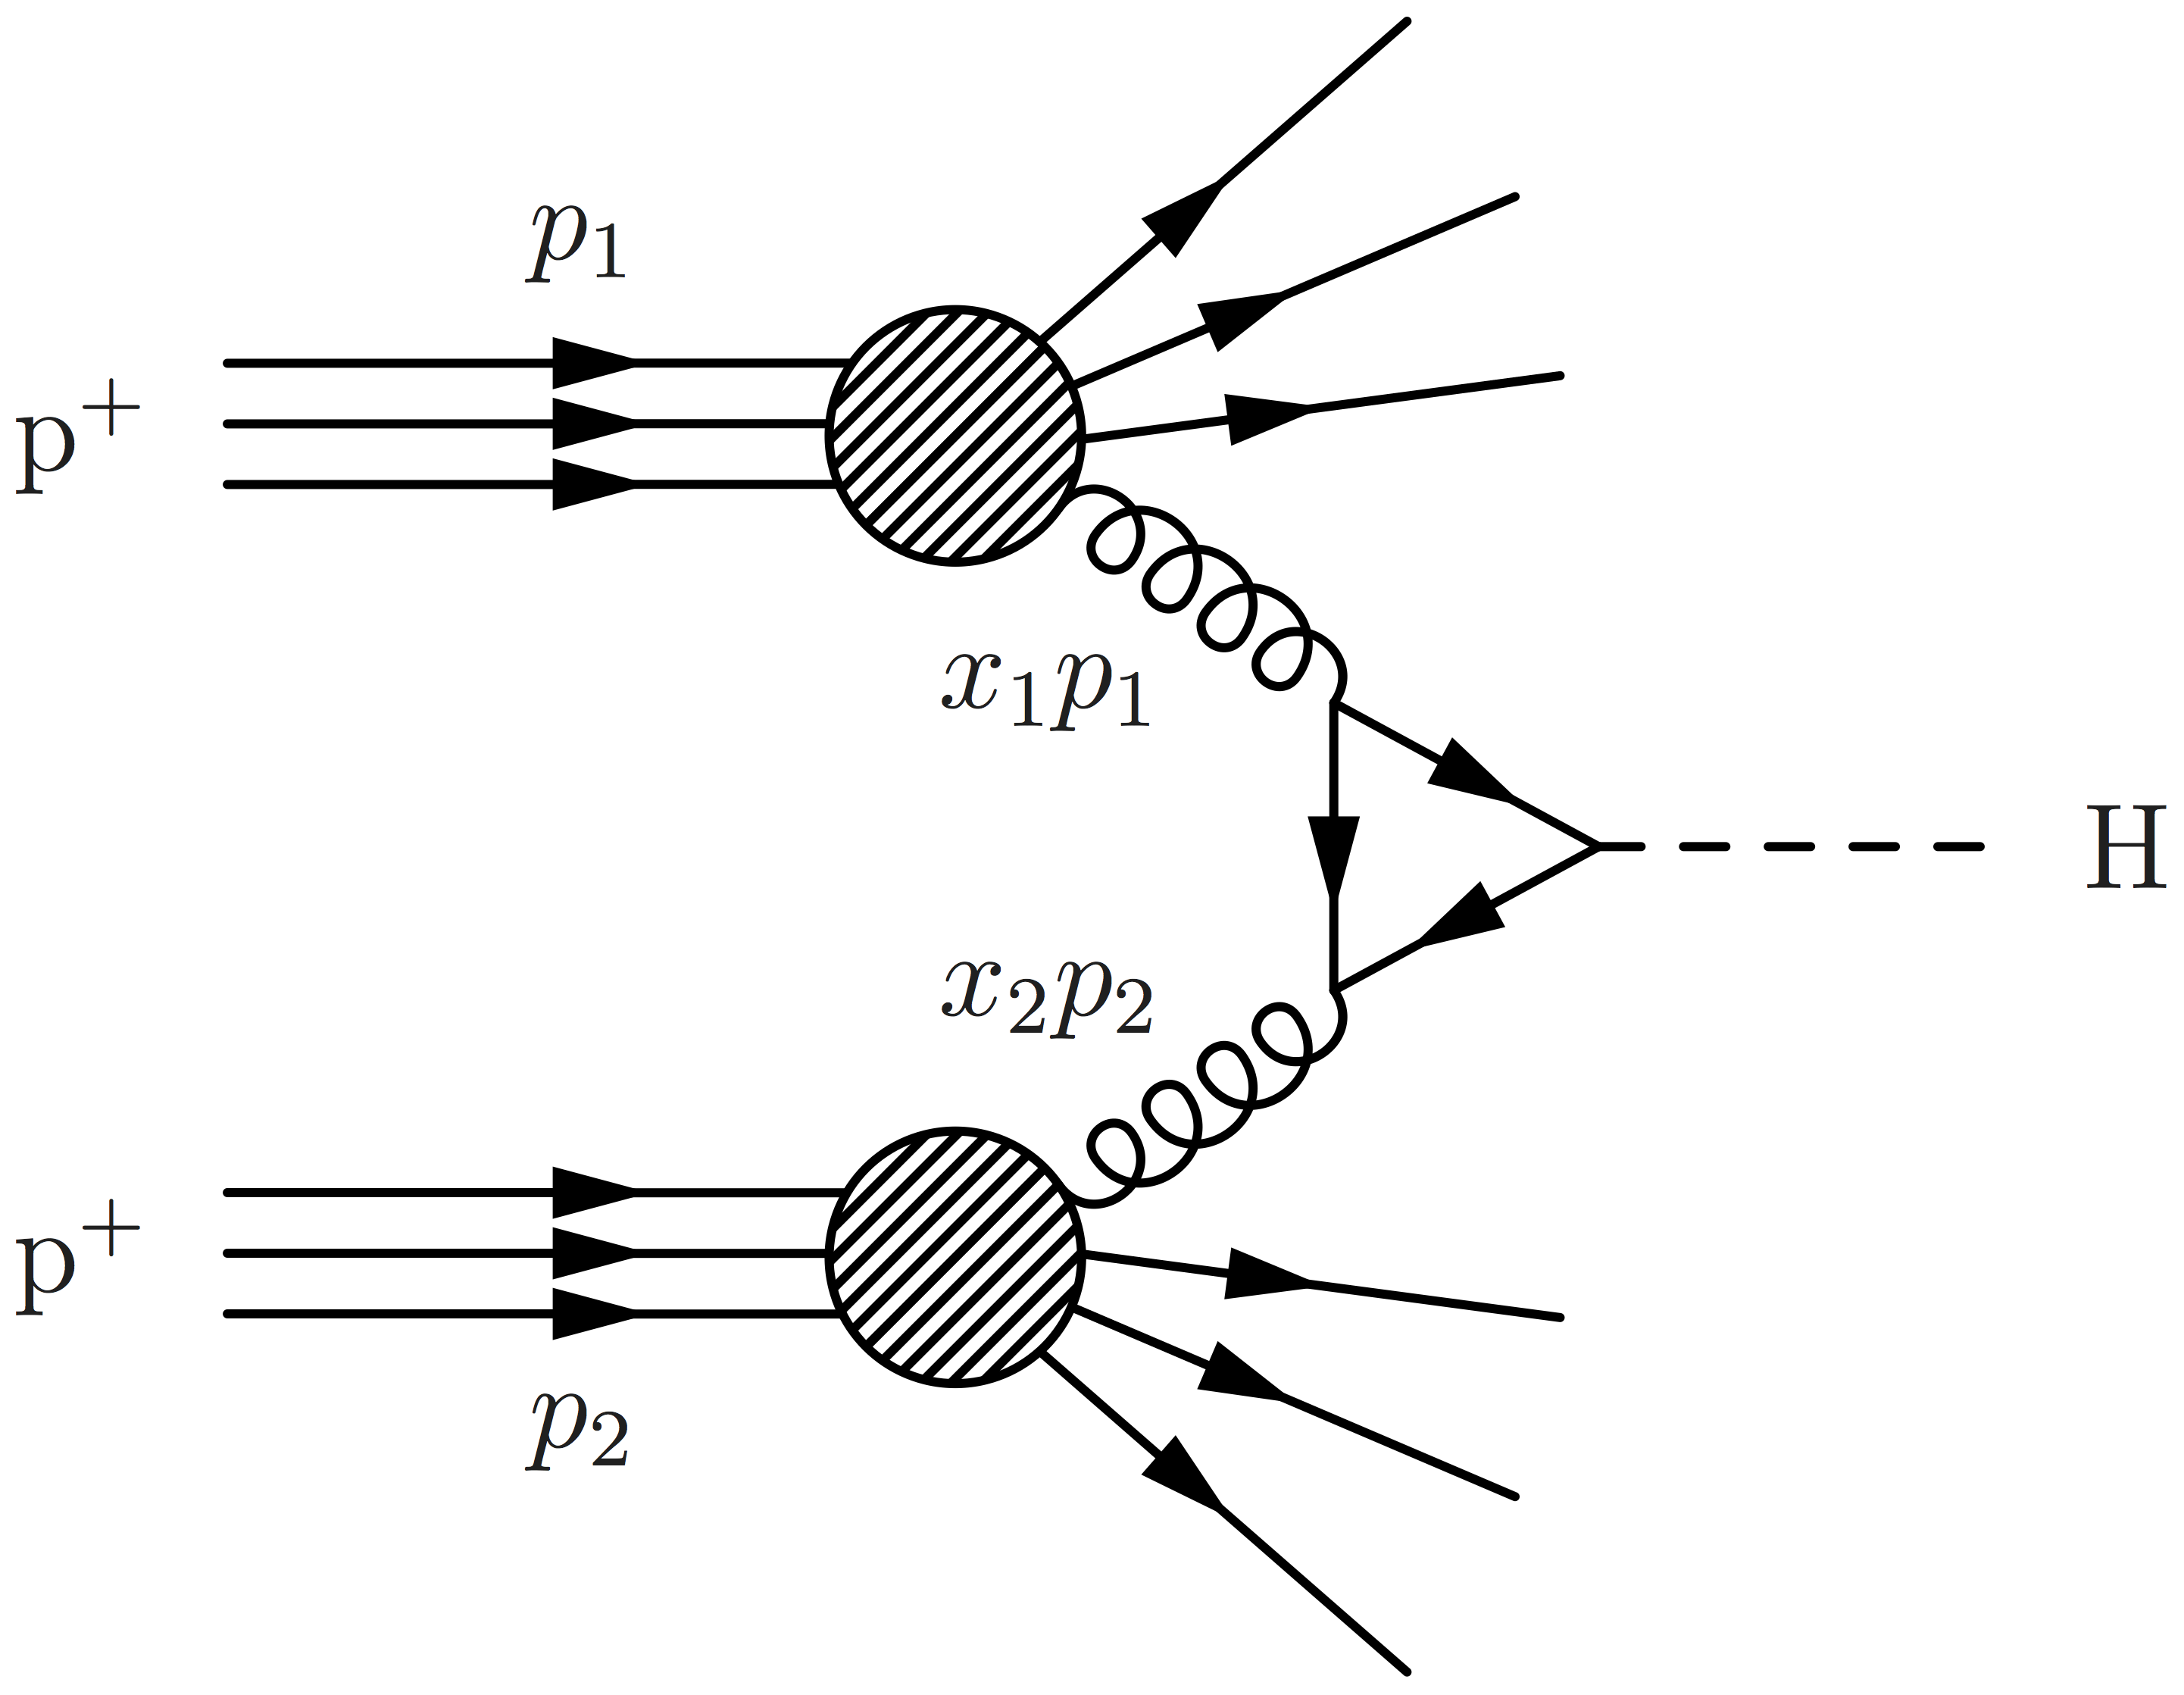
\includegraphics[width=0.6\textwidth]{ch-qcd/ggh}
	\caption{
		The \lo Feynman diagram associated to the scattering of two gluon
		components of the proton, coupling to a virtual quark loop, that
		finally generates an Higgs boson.
		This is the Higgs production via gluon fusion, the main channel for
		Higgs production at \lhc.
	}
	\label{fig:qcd/ggh}
\end{figure}

New processes and observables are being observed at the \lhc, possibly
including new particles and new physics, stressing the need for a more precise
determination of the proton structure.
%
The Higgs production, whose main channel is represented in \cref{fig:qcd/ggh},
that has been first detected by the \lhc collaborations \atlas
\cite{ATLAS:2012yve} and \cms \cite{CMS:2012qbp}, is an extremely well-known
example of new particle discovery, which heavily involved a proton initiated
process, thus depending critically on the \pdf{}s knowledge.
